\documentclass[a4paper]{report}\usepackage[]{graphicx}\usepackage[]{color}
%% maxwidth is the original width if it is less than linewidth
%% otherwise use linewidth (to make sure the graphics do not exceed the margin)
\makeatletter
\def\maxwidth{ %
  \ifdim\Gin@nat@width>\linewidth
    \linewidth
  \else
    \Gin@nat@width
  \fi
}
\makeatother

\definecolor{fgcolor}{rgb}{0.345, 0.345, 0.345}
\newcommand{\hlnum}[1]{\textcolor[rgb]{0.686,0.059,0.569}{#1}}%
\newcommand{\hlstr}[1]{\textcolor[rgb]{0.192,0.494,0.8}{#1}}%
\newcommand{\hlcom}[1]{\textcolor[rgb]{0.678,0.584,0.686}{\textit{#1}}}%
\newcommand{\hlopt}[1]{\textcolor[rgb]{0,0,0}{#1}}%
\newcommand{\hlstd}[1]{\textcolor[rgb]{0.345,0.345,0.345}{#1}}%
\newcommand{\hlkwa}[1]{\textcolor[rgb]{0.161,0.373,0.58}{\textbf{#1}}}%
\newcommand{\hlkwb}[1]{\textcolor[rgb]{0.69,0.353,0.396}{#1}}%
\newcommand{\hlkwc}[1]{\textcolor[rgb]{0.333,0.667,0.333}{#1}}%
\newcommand{\hlkwd}[1]{\textcolor[rgb]{0.737,0.353,0.396}{\textbf{#1}}}%
\let\hlipl\hlkwb

\usepackage{framed}
\makeatletter
\newenvironment{kframe}{%
 \def\at@end@of@kframe{}%
 \ifinner\ifhmode%
  \def\at@end@of@kframe{\end{minipage}}%
  \begin{minipage}{\columnwidth}%
 \fi\fi%
 \def\FrameCommand##1{\hskip\@totalleftmargin \hskip-\fboxsep
 \colorbox{shadecolor}{##1}\hskip-\fboxsep
     % There is no \\@totalrightmargin, so:
     \hskip-\linewidth \hskip-\@totalleftmargin \hskip\columnwidth}%
 \MakeFramed {\advance\hsize-\width
   \@totalleftmargin\z@ \linewidth\hsize
   \@setminipage}}%
 {\par\unskip\endMakeFramed%
 \at@end@of@kframe}
\makeatother

\definecolor{shadecolor}{rgb}{.97, .97, .97}
\definecolor{messagecolor}{rgb}{0, 0, 0}
\definecolor{warningcolor}{rgb}{1, 0, 1}
\definecolor{errorcolor}{rgb}{1, 0, 0}
\newenvironment{knitrout}{}{} % an empty environment to be redefined in TeX

\usepackage{amsmath}
\usepackage{alltt}
\usepackage[fontsize=13pt]{scrextend}
\usepackage[utf8]{vietnam}
\usepackage{verbatim} 
\usepackage{lipsum}
\usepackage{listings}



\makeatletter
\title{Ứng dụng, đánh giá, và so sánh một số mô hình phân loại vào việc phân loại khách hàng thẻ tín dụng}\let\Title\@title
\author{Nguyễn Đức Hiếu}\let\Author\@author
\makeatother
%%%%%%%%%%%%%%%%%%%%%%%%%
% TITLE PAGE FORMATTING %
%%%%%%%%%%%%%%%%%%%%%%%%%
\usepackage{afterpage}
\usepackage{xcolor}
\usepackage{graphicx}

%%%%%%%%%%%%%%%%%%%%%%%%
% PARAGRAPH FORMATTING %
%%%%%%%%%%%%%%%%%%%%%%%%
\usepackage{enumitem}
% Indent first paragraphs after each sections
\usepackage{indentfirst}

% Document formatting
\usepackage{mathptmx}
\renewcommand{\baselinestretch}{1.3}
\usepackage[a4paper]{geometry}
  \geometry{
  top=25mm,
  left=35mm,
  bottom=25mm,
  right=25mm
  }
%%%%%%%%%%%%%%%%%%%%%
% HEADER AND FOOTER %
%%%%%%%%%%%%%%%%%%%%%
\usepackage{etoolbox}
\patchcmd{\chapter}{\thispagestyle{plain}}{\thispagestyle{fancy}}{}{}
\usepackage{fancyhdr}
\pagestyle{fancy}
\fancyhf{}
\lhead{}
\chead{\normalsize Chuyên đề thực tập chuyên ngành Toán Kinh tế}
\rhead{}
\lfoot{}
\cfoot{\normalsize 11131371 - Nguyễn Đức Hiếu}
\rfoot{\normalsize Trang \thepage}
\renewcommand{\headrulewidth}{0.4pt}
\renewcommand{\footrulewidth}{0.4pt}
%%%%%%%%%%%%%%%%%%%%%%
% SECTION FORMATTING %
%%%%%%%%%%%%%%%%%%%%%%


\usepackage{titlesec}

\titleformat{\chapter}[display]
{\centering\Large\bfseries}
{\MakeUppercase{\chaptertitlename}  \thechapter}{1em}
{\MakeUppercase}

\titleformat{name=\chapter,numberless}[display]
  {\normalfont\Large\bfseries\filcenter}{}{1ex}
  {\MakeUppercase}[\vspace{1ex}]

\titleformat{\section}[hang]
{\bfseries}
{\thesection}{1em}
{\MakeUppercase}

\titleformat{\subsection}[hang]
{\bfseries}
{\thesubsection}{1em}
{}

%%%%%%%%%%%%%%%%%%%%%%  
% FIGURES AND TABLES %
%%%%%%%%%%%%%%%%%%%%%%
\usepackage[section]{placeins}
\usepackage[justification=centering]{caption}

%%%%%%%%%%%%%%%%%%%
% TOC FORMATTING  %
%%%%%%%%%%%%%%%%%%%

% Package hyperref should be loaded last, as it rewrites many commands.
% \usepackage{tocloft}
\usepackage[colorlinks=true, citecolor=blue, linkcolor=blue]{hyperref}
\usepackage[all]{hypcap}
% Customise for table of contents labeling
\setcounter{tocdepth}{3}
\setcounter{secnumdepth}{4}
%%%%%%%%%%%%
% CITATION %
%%%%%%%%%%%%
% Setting up for citation styles
% \usepackage{natbib}
\usepackage[backend=bibtex,bibstyle=luanan,sorting=ydnt,style=authoryear]{biblatex}
\addbibresource{reference.bib}
% Add number to bibliography
\defbibenvironment{bibliography}
  {\enumerate
     {}
     {\setlength{\leftmargin}{\bibhang}%
      \setlength{\itemindent}{-\leftmargin}%
      \setlength{\itemsep}{\bibitemsep}%
      \setlength{\parsep}{\bibparsep}}}
  {\endenumerate}
  {\item}
%%%%%%%%%%%%%%%%%%%%%%%%%%%%%%%%%%%%%%%%%%%%
%%%%%%%%%%%%%%%%%%%%%%%%%%%%%%%%%%%%%%%%%%%%
%%%%---------DOCUMENT CONTENTS----------%%%%
%%%%%%%%%%%%%%%%%%%%%%%%%%%%%%%%%%%%%%%%%%%%
%%%%%%%%%%%%%%%%%%%%%%%%%%%%%%%%%%%%%%%%%%%%
\IfFileExists{upquote.sty}{\usepackage{upquote}}{}
\begin{document}
%%%%%%%%%%%%%%%%%%%%%%%%%%%%%%%
%         TITLE PAGE          %
%%%%%%%%%%%%%%%%%%%%%%%%%%%%%%%
\begin{titlepage}

\definecolor{titlepagecolor}{RGB}{1, 81, 159 }
% \definecolor{titlepagecolor}{RGB}{128, 0, 0 }
\color{white}
\pagecolor{titlepagecolor}\afterpage{\nopagecolor}
\large
\centering
\textbf{TRƯỜNG ĐẠI HỌC KINH TẾ QUỐC DÂN}

\textbf{KHOA TOÁN KINH TẾ}
\vspace{5mm}


\includegraphics[width=0.4\textwidth]{./Cover/neu-logo.png}\par\vspace{1cm}
{\bfseries\scshape\Huge Chuyên đề thực tập}


\begin{description}[leftmargin=6cm,style=nextline]
\item[Chuyên ngành:] Toán Kinh tế
\item[Đề tài:] \Title
\item[Sinh viên thực hiện:] Nguyễn Đức Hiếu
\item[Mã sinh viên:] 11131371
\item[Lớp:] Toán Kinh tế 55
\item[Giảng viên hướng dẫn:] PGS. Nguyễn Thị Minh
\end{description}

\centering
\vfill
% Bottom of the page
\makebox[0pt]{\rule{0.5\textwidth}{1pt}}

{\large Hà Nội,  \today\par}
\end{titlepage}


%%%%%%%%%%%%%%%
% Lời mở đầu %
%%%%%%%%%%%%%%%
\chapter*{Lời mở đầu}
\addcontentsline{toc}{chapter}{Lời mở đầu}

% LỜI MỞ ĐẦU  
%
% - Nêu vấn đề
Đối với các ngân hàng việc chấm điểm tín dụng và phân loại các khách hàng là yếu tố thiết yếu cho lợi nhuận của ngân hàng.
%
Phương pháp truyền thống của việc ra quyết định có cho một cá nhân cụ thể vay hay không là dựa trên đánh giá cảm tính dựa trên kinh nghiệm cá nhân.
%
Tuy nhiên, sự phát triển về quy mô của nền kinh tế đã tạo ra sức ép về nhu cầu vay, đi kèm với đó là sự cạnh tranh giữa các ngân hàng và công nghệ máy tính ngày càng phát triển đã khiến cho việc sử dụng các mô hình thống kê trong việc phân loại các khách hàng tín dụng là bắt buộc đối với các ngân hàng trên thế giới mà ở Việt Nam cũng không phải là ngoại lệ.
%

Vậy, phương pháp ước lượng nào có thể giúp chúng ta xây dựng được hệ thống chấm điểm tín dụng chính xác nhất? Đã có một số nghiên cứu mang tính chất so sánh hiệu năng giữa các mô hình \parencite{baesens2003benchmarking, xiao2006comparative, lessmann2015benchmarking}. 
Sự khác biệt về hiệu năng của các phương pháp khác nhau là có, tuy nhiên hầu như là không đáng kể, và không phải các mô hình hiệu quả hơn đều là các mô hình mới và tân tiến.
Theo \textcite{thomas2010consumer}, cách hiệu quả để xây dựng một hệ thống lượng định hiệu quả là phối hợp nhiều mô hình khác nhau thay vì tìm kiếm một mô hình toàn diện có thể áp dụng với tất cả các ngân hàng.

Trong bài này, chúng ta sẽ tiếp cận đến một số phương pháp phân loại các khách hàng tín dụng phổ biến hiện nay và rút ra một số kết luận về việc sử dụng các phương pháp khác nhau sao cho hợp lý. Bài viết này được bố cục như sau:

\begin{itemize}
\item \textbf{Chương 1} đưa ra một cái nhìn tổng quan về lĩnh vực quản trị rủi ro tín dụng trong ngân hàng và đưa ra một số vấn đề của việc chấm điểm tín dụng tại các ngân hàng Việt Nam.
\item Các mô hình được thực hiện trong bài này sẽ được giới thiệu ở \textbf{Chương 2}, đi kèm với đó là một số chỉ tiêu sẽ được dùng để đánh giá mô hình trong bài này.
\item Trong \textbf{Chương 3}, chúng ta sẽ ứng dụng các phương pháp được giới thiệu ở \textbf{Chương 2} trong một bộ số liệu mẫu về các khách hàng thẻ tín dụng trong một ngân hàng ở Đài Loan.
\item Kết quả của các mô hình sẽ được thảo luận ở \textbf{Chương 4}, cùng với một số kết luận rút ra được sau khi áp dụng mô hình.
\end{itemize}

% - Hướng tiếp cận 
Đề tài này được soạn thảo bằng \LaTeX{} kết hợp với \texttt{Sweave} và \texttt{knitr} 
\parencite{r:knitr}. Tất cả phân tích được thực hiện trên phần mềm thống kê 
R version 3.3.3 (2017-03-06) \parencite{r:rbase},  
các phân tích cụ thể được thực hiện sử dụng các gói mở rộng \texttt{caret}\parencite{r:caret}, \texttt{glmnet}\parencite{r:glmnet}, \texttt{tidyverse} \parencite{r:tidyverse}... 

%  Cảm ơn bla bla
Em xin cảm ơn giáo viên hướng dẫn, cô Nguyễn Thị Minh, trưởng khoa 
Toán Ứng dụng trong Kinh tế, cùng với các thầy cô giáo khác trong khoa đã tạo điều kiện cho em thực hiện đề tài này.
%%%%%%%
% TOC %
%%%%%%%
\clearpage\tableofcontents
\addcontentsline{toc}{chapter}{Mục lục}

\listoftables
\addcontentsline{toc}{chapter}{Danh sách bảng}

\listoffigures
\addcontentsline{toc}{chapter}{Danh sách hình}

%%%%%%%%%%%%
% Chương 1 %
%%%%%%%%%%%%
\chapter{Tổng quan về quản trị rủi ro tín dụng đối với khách hàng cá nhân}

\section{Một số khái niệm}

\section{Thực trạng của việc chấm điểm tín dụng tại Việt Nam}

\section{Kết luận}

%%%%%%%%%%%%
% Chương 2 %
%%%%%%%%%%%%

\chapter{Các phương pháp phân loại khách hàng vay thẻ tín dụng}
\section{Các mô hình phân loại}

\subsection{Mô hình logit}

\subsubsection{Khái niệm}

Mô hình hồi quy Logistic (hay logit) được dùng để nghiên cứu mối quan hệ giữa xác suất của các biến nhị phân hoặc phân loại và các biến giải thích khác. Hướng tiếp cận của mô hình Logistic cho bài toán phân loại là bằng cách ước lượng giá trị xác suất $P(y = 1|X)$ như sau:

{\large
$$
P(y = 1|X) = \frac{e^{\beta_0 + \sum\beta_1X_1 +\beta_2X_2 + \ldots + \beta_nX_n}}{1 + e^{\beta_0 + \sum\beta_1X_1 +\beta_2X_2 + \ldots + \beta_nX_n}}
$$
}

Với $y$ là biến dùng để phân loại, chỉ nhận hai giá trị 0 hoặc 1, $X$ là các vector của biến độc lập, $\beta_0$, $\beta_1$, $\beta_2$, ..., $\beta_n$ là các hệ số cần ước lượng. 

Hay còn được viết dưới dạng:

{\large
$$
\log\frac{P(y = 1|X)}{P(y = 0|X)} = \beta_0 + \beta_1X_1 +\beta_2X_2 + \ldots + \beta_nX_n
$$
}

% Trong đó giá trị $\log [P(y = 1|X)/P(y = 0|X) ]$ còn được gọi là 
 
%If some of the independent variables are discrete, nominal scale variables such as race, sex, treatment group, and so forth, it is inappropriate to include them in the model as if they were interval scale variables. The numbers used to represent the various levels of these nominal scale variables are merely identifiers, and have no numeric significance. In this situation, the method of choice is to use a collection of design variables (or dummy variables). Suppose, for example, that one of the independent variables is race, which has been coded as “white,” “black,” and “other.” In this case, two design variables are necessary. One possible coding strategy is that when the respondent is “white,” the two design variables, D 1 and D 2 , would both be set equal to zero; when the respondent is “black,” D 1 would be set equal to 1 while D 2 would still equal 0; when the race of the respondent is “other,” we would use D 1 = 0 and D 2 = 1.
Trong trường hợp các biến độc lập là biến phân loại không so sánh được (ví dụ: Giới tính, dân tộc, v..v..) chúng ta đưa các biến này vào mô hình bằng cách sử dụng một nhóm các biến giả tương ứng với từng giá trị khác nhau của biến phân loại.

\subsubsection{Ước lượng mô hình logit}
a, Ước lượng hợp lý tối đa

\vspace{5mm}

%Logistic regression models are usually fit by maximum likelihood, using the conditional likelihood of G given X. Since Pr(G|X) completely specifies the conditional distribution, the multinomial distribution is appropriate. The log-likelihood for N observations is

Các hệ số $\beta$ thường được ước lượng bằng phương pháp ước lượng hợp lý tối đa \parencite{hosmer2013applied}, sử dụng hàm hợp lý có điều kiện $G$ đối với mỗi giá trị của $X$. Hàm hợp lý logarit cho $N$ quan sát được viết như sau:

{\large

$$
L(\theta) = \sum_{i = 1}^N P_{g_i} (x_i; \theta)
$$
}
, với $p_k(x_i;\theta) = P(G = k|X = x_i; \theta)$.

Trong trường hợp biến phụ thuộc $Y$ chỉ có 2 giá trị: $(0, 1)$, ta có thể mã hóa 2 nhóm của $g_i$ thành$y_i = 1$ khi $g_i = 1$ và $y_i = 0$ khi $g_i = 2$. Khi đó logarit của hàm hợp lý có thể viết lại như  sau: 

{\large
$$
L(\beta) = \sum_{i = 1}^N \{  y_i log (x_i ; \beta) + (1- y_i)log (x_i; \beta) \}
$$
}

Tối ưu hóa hàm $L$ sẽ cho chúng ta ước lượng hợp lý tối đa cho các hệ số $\beta$ trong mô hình.

b, Ràng buộc L1 hay mô hình Lasso

\vspace{5mm}

Một vấn đề mô hình logit hay gặp phải đó là hiện tượng đa cộng tuyến giữa các biến khi số lượng biến $p$ tăng lên. Hậu quả của hiện tượng này là các ước lượng cho hệ số $\beta$ thường là có sai số lớn, mặc dù ước lượng vẫn là không chệch. Nói cách khác, các giá trị $\beta$ ước lượng được thường có hiệu quả kém khi áp dụng trên mẫu mới, mặc dù mô hình vẫn có độ chính xác cao khi áp dụng trên bộ số liệu mẫu dùng để ước lượng ra mô hình. 

Để xử lý vấn đề này, chúng ta có thể áp dụng nhiều phương pháp để loại biến ra khỏi mô hình, hoặc sử dụng các phương pháp ước lượng khác mà các biến có ý nghĩa thống kê thấp bị loại ra khỏi mô hình trong quá trình ước lượng.

Phương pháp Lasso là một cải tiến của các mô hình tuyến tính, trong mô hình này, chúng ta áp dụng thêm ràng bộc L1 đối với hàm hợp lý tối đa. Áp dụng với mô hình Logit, thay vì tối ưu hàm hợp lý tối đa, chúng ta tối ưu:

{\large
$$
\max_{\beta_0, \beta} \left \{ \sum_{i = 1}^N [ y_i log (x_i ; \beta) + (1- y_i)log (x_i; \beta)] - \lambda \sum_{j = 1}^p|\beta_j|\right \}
$$
}

%As with the lasso, we typically do not penalize the intercept term, and stan-dardize the predictors for the penalty to be meaningful. Criterion (4.31) is126 concave, and a solution can be found using nonlinear programming meth-ods (Koh et al., 2007, for example). Alternatively, using the same quadratic approximations that were used in the Newton algorithm in Section 4.4.1, we can solve (4.31) by repeated application of a weighted lasso algorithm. Interestingly, the score equations [see (4.24)] for the variables with non-zero coefficients have the form
Sử dụng các giá trị khác nhau của tham số $\lambda$, phương pháp lasso thu nhỏ giá trị ước lượng của các $\beta$ so với phương pháp tối đa hóa hàm hợp lý truyền thống. Vì các giá trị thu nhỏ của $\beta$ có thể giảm về 0 và loại ra khỏi mô hình nếu $\lambda$ đủ lớn, phương pháp lasso có thể được dùng để thay thế cho việc chọn biến trong các mô hình đa biến.

Đồng thời đối với lasso, ta thường không ràng buộc các hệ số chặn, và các biến giải thích phải được chuẩn hóa để ràng buộc chung cho các $\beta$ là có ý nghĩa. Vì hàm tối ưu của chúng ta là hàm lõm, lời giải có thể tính sử dụng các phương pháp phi tuyến. %need citation


\subsubsection{Diễn giải kết quả ước lượng mô hình}

\subsection{Mô hình phân loại tuyến tính}
\subsection{Mô hình SVM (Support Vector Machine)}

\section{Đánh giá mô hình}
\subsection{Đường ROC và phần diện tích dưới đường cong (AUC)}
\subsection{Thang đo H}

%%%%%%%%%%%%
% Chương 3 %
%%%%%%%%%%%%

\chapter{Tình huống nghiên cứu}

\section{Số liệu và các biến số}

Chúng ta thực hành trên bộ số liệu mẫu bao gồm 30000 quan sát và 25 biến bao gồm tình trạng trả nợ, các thông tin nhân khẩu học cơ bản cùng với số liệu về tín dụng và tình trạng hồ sơ của các khách hàng thẻ tín dụng ở Đài Loan từ tháng 4 năm 2005 đến tháng 9 năm 2005.

Các tên biến đã được thay đổi để tiện lợi cho việc đọc hiểu và phân tích, cụ thể như sau:

\begin{description}
  \item [\texttt{ID}] Số ID của mỗi khách hàng tín dụng
  \item [\texttt{LIMIT\_BAL}] Lượng tín dụng cho vay tính bằng Đô la Đài Loan (bao gồm cả các khoản vay cá nhân và các khoản vay với thẻ tín dụng phụ)
  \item [\texttt{SEX}] Giới tính (0=Nữ, 1=Nam)
  \item [\texttt{EDUCATION}] (1=sau đại học, 2=đại học, 3=phổ thông, 4=khác)
  \item [\texttt{MARRIAGE}] Trạng thái hôn nhân (1=đã cưới, 2=độc thân, 3=khác)
  \item [\texttt{AGE}] Số tuổi tính bằng năm
  \item [\texttt{PAY\_0}] Tình trạng hồ sơ vào thời điểm tháng 9/2005 (-1=trả đúng hạn, 1=chậm 1 tháng, 2=chậm 2 tháng, ... 8=chậm 8 tháng, 9=chậm 9 tháng hoặc nhiều hơn)
  \item [\texttt{PAY\_2}] Tình trạng hồ sơ vào thời điểm tháng 8/2005 (thang điểm như trên)
  \item [\texttt{PAY\_3}] Tình trạng hồ sơ vào thời điểm tháng 7/2005 (thang điểm như trên)
  \item [\texttt{PAY\_4}] Tình trạng hồ sơ vào thời điểm tháng 6/2005 (thang điểm như trên)
  \item [\texttt{PAY\_5}] Tình trạng hồ sơ vào thời điểm tháng 5/2005 (thang điểm như trên)
  \item [\texttt{PAY\_6}] Tình trạng hồ sơ vào thời điểm tháng 4/2005 (thang điểm như trên)
  \item [\texttt{BILL\_AMT1}] Hóa đơn thanh toán vào thời điểm 9/2005 (Đô la Đài Loan)
  \item [\texttt{BILL\_AMT2}] Hóa đơn thanh toán vào thời điểm 8/2005 (Đô la Đài Loan)
  \item [\texttt{BILL\_AMT3}] Hóa đơn thanh toán vào thời điểm 7/2005 (Đô la Đài Loan)
  \item [\texttt{BILL\_AMT4}] Hóa đơn thanh toán vào thời điểm 6/2005 (Đô la Đài Loan)
  \item [\texttt{BILL\_AMT5}] Hóa đơn thanh toán vào thời điểm 5/2005 (Đô la Đài Loan)
  \item [\texttt{BILL\_AMT6}] Hóa đơn thanh toán vào thời điểm 4/2005 (Đô la Đài Loan)
  \item [\texttt{PAY\_AMT1}] Lượng tiền đã thanh toán vào thời điểm tháng 9/2015 (Đô la Đài Loan)
  \item [\texttt{PAY\_AMT2}] Lượng tiền đã thanh toán vào thời điểm tháng 8/2015 (Đô la Đài Loan)
  \item [\texttt{PAY\_AMT3}] Lượng tiền đã thanh toán vào thời điểm tháng 7/2015 (Đô la Đài Loan)
  \item [\texttt{PAY\_AMT4}] Lượng tiền đã thanh toán vào thời điểm tháng 6/2015 (Đô la Đài Loan)
  \item [\texttt{PAY\_AMT5}] Lượng tiền đã thanh toán vào thời điểm tháng 5/2015 (Đô la Đài Loan)
  \item [\texttt{PAY\_AMT6}] Lượng tiền đã thanh toán vào thời điểm tháng 4/2015 (Đô la Đài Loan)
  \item [\texttt{DEFAULT}] Có trả nợ hay không (1=có, 0=không)
\end{description}


Hình \ref{fig:corr_mat} (trang \pageref{fig:corr_mat}) mô tả ma trận hệ số tương quan Pearson giữa các biến số trong bộ số liệu. 
Lưu ý tương quan giữa các biến trong nhóm biến \texttt{PAY} (tình trạng hồ sơ) và 
giữa các biến trong nhóm biến \texttt{BILL\_AMT} (hoá đơn thanh toán) là khá cao, thể hiện sự tương đồng cao về mặt thông tin thể hiện của các biến này.
Trong số các biến trong bộ số liệu, các biến \texttt{PAY} là có thể hiện tương quan dương với biến \texttt{DEFAULT}, gợi ý rằng chúng ta có thể sử dụng biến này là biến chính để dự đoán tỉ lệ vỡ nợ của khách hàng.

\begin{figure}[h]
\centering
\capstart
\begin{knitrout}\small
\definecolor{shadecolor}{rgb}{0.969, 0.969, 0.969}\color{fgcolor}
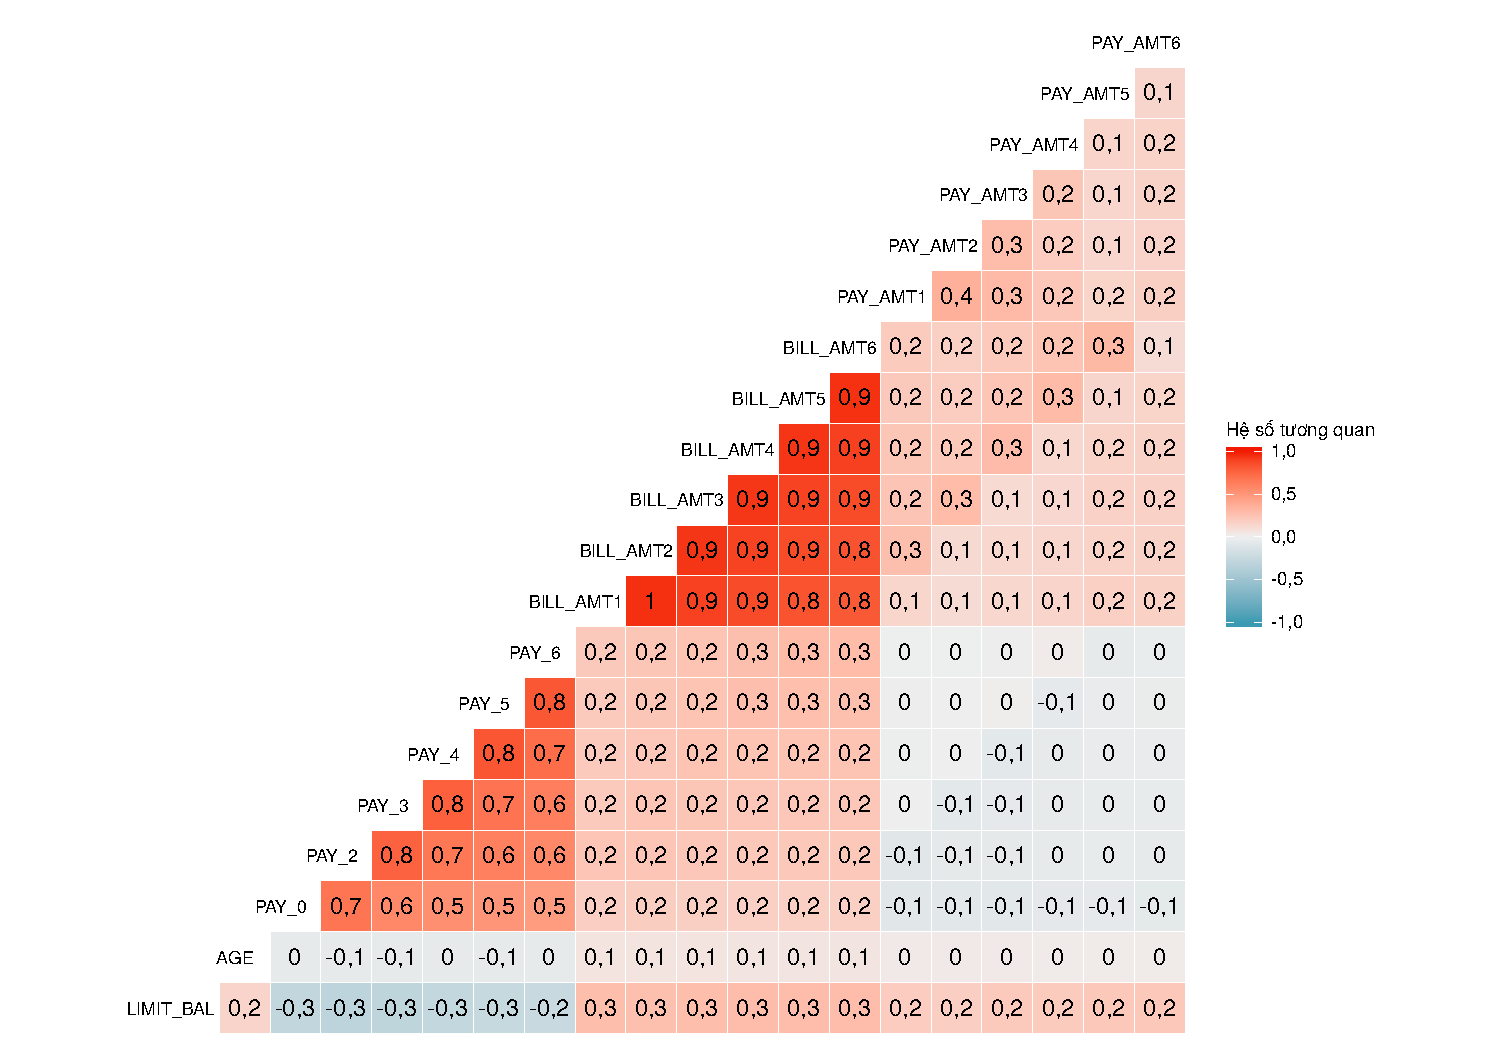
\includegraphics[width=\textwidth]{Figures/corr_mat-1} 

\end{knitrout}
\caption[Ma trận hệ số tương quan Pearson]{Ma trận hệ số tương quan Pearson giữa các biến trong bộ số liệu.}
\label{fig:corr_mat}
\end{figure}

Để có cái nhìn cụ thể hơn vào bộ số liệu này, chúng ta sử dụng phương pháp phân tích thành phần chính (PCA - Principal Component Analysis) để phân tích bộ số liệu.
Với phương pháp này, chúng ta tìm một hệ tọa độ trực giao mới để thể hiện bộ số liệu, sao cho với thành phần chính thứ nhất (chiều thứ nhất của hệ tọa độ mới) thể hiện được nhiều nhất có thể thông tin của bộ số liệu, thành phần chính thứ hai (chiều thứ hai của hệ tọa độ mới) thể hiện nhiều nhất có thể lượng thông tin còn lại của bộ số liệu, v...v... Lưu ý rằng vì các biến trong bộ số liệu có thang đo khác nhau, để đảm bảo hiệu quả cho phương pháp phân tích đa biến này, chúng ta chuẩn hóa các biến trước khi thực hiện PCA. Đồng thời, các biến phân loại như \texttt{EDUCATION} và \texttt{MARRIAGE} cũng được lược bỏ.

\begin{figure}[h]
\centering
\capstart
\begin{knitrout}\small
\definecolor{shadecolor}{rgb}{0.969, 0.969, 0.969}\color{fgcolor}
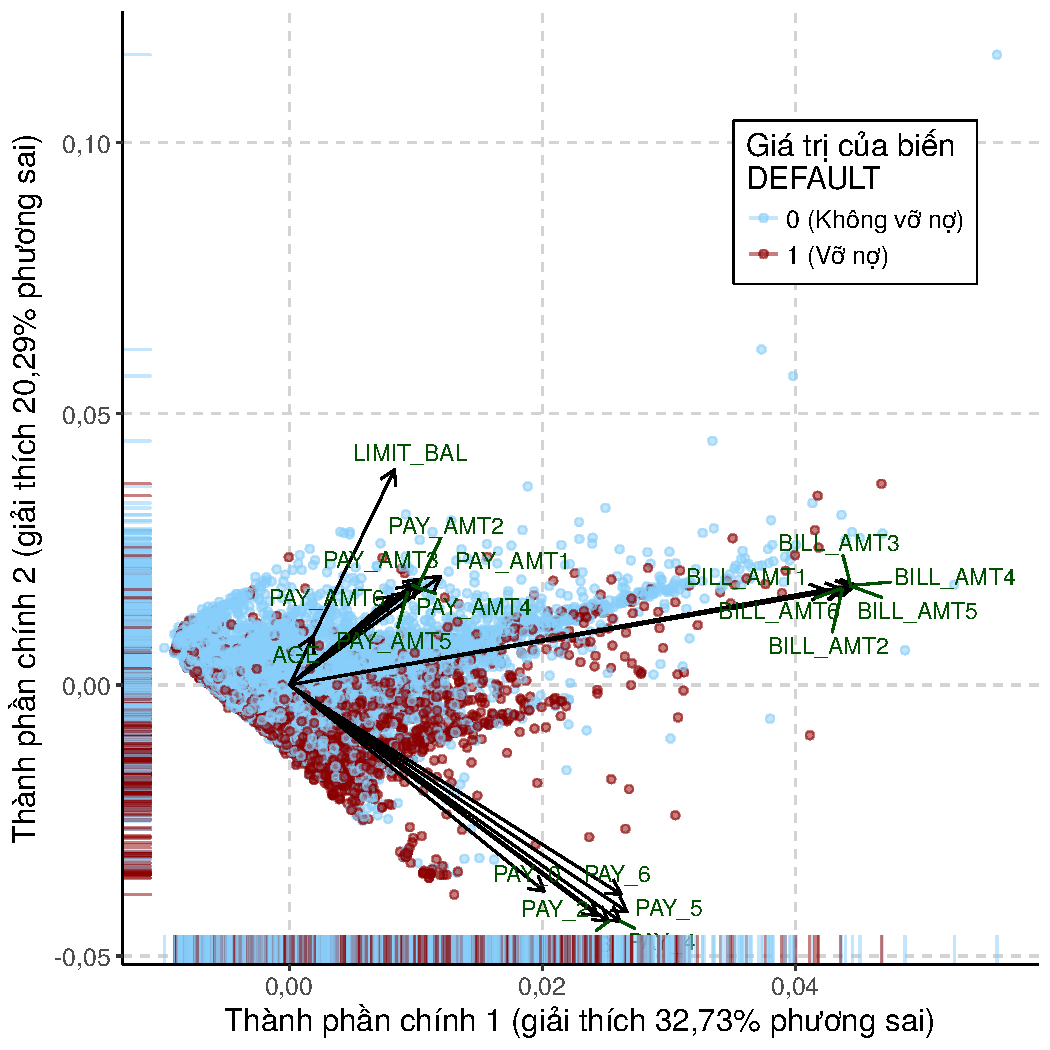
\includegraphics[width=10cm,height=10cm]{Figures/pca-1} 

\end{knitrout}
\caption{Phép chiếu bộ số liệu trên hai thành phần chính.}
\label{fig:pca}
\end{figure}

Phép chiếu của các biến và các quan sát trong bộ số liệu trên hai thành phần chính đầu tiên được thể hiện trong hình \ref{fig:pca} (trang \pageref{fig:pca}), với mỗi véc tơ thể hiện một biến và mỗi điểm thể hiện một quan sát trong bộ số liệu. Các quan sát thuộc vào nhóm vỡ nợ (biến \texttt{DEFAULT} bằng 1) có màu đỏ và các quan sát thuộc nhóm không vỡ nợ (biến \texttt{DEFAULT} bằng 0) có màu xanh. 
Quan sát đồ thị này, chúng ta nhận thấy các quan sát thuộc nhóm vỡ nợ (màu đỏ) tập trung nhiều ở phía dưới đồ thị, hay là giá trị của các biến này chiếu trên thành phần chính thứ 2 (trục tung) là thấp hơn. 
Như chúng ta nhận xét ở ma trận hệ số tương quan phía trên, véc tơ chiếu các biến thuộc cùng nhóm \texttt{PAY}, \texttt{PAY\_ATM} và \texttt{BILL\_ATM} nằm khá gần nhau, thể hiện mức độ tương quan cao giữa các biến số thuộc cùng một trong ba nhóm này. Các biến thuộc nhóm \texttt{PAY} có hướng trùng với hướng phân bố của các quan sát thuộc nhóm vỡ nợ, trong khi các biến thuộc nhóm \texttt{PAY\_ATM} có hướng trùng với hướng phân bố của các quan sát thuộc nhóm không vỡ nợ, gợi ý tiềm năng dùng để dự báo của các nhóm biến này. 
Ngoài ra các quan sát nhóm vỡ nợ cũng có xu hướng thể hiện cao trên biến 
\texttt{SEX}. Nhóm các quan sát không vỡ nợ cũng phân bố nhiều theo chiều tăng của các biến \texttt{AGE} và \texttt{LIMIT\_BAL}.

Lưu ý rằng đồ thị \ref{fig:pca} chỉ thể hiện $\text{53,02}$ phần trăm lượng thông tin của bộ số liệu, chưa kể các biến phân loại như \texttt{EDUCATION} hay \texttt{MARRIAGE}. Bằng cách sử dụng các phương pháp phân tích cụ thể hơn, chúng ta có thể đưa ra một mô hình phân loại chính xác hơn đối với khả năng vỡ nợ của các khách hàng dùng thẻ tín dụng trong bộ số liệu này.

Trong 30000 quan sát của bộ số liệu này, sau khi làm sạch, chúng ta chọn ngẫu nhiên 75\% (Khoảng hơn 22000 quan sát) để xây dựng các mô hình. Số lượng quan sát còn lại sẽ được dùng để kiểm tra các mô hình xây dựng được và cho chúng ta cái nhìn về hiệu quả của chúng.


\section{Ứng dụng mô hình logit}

\subsection{Tiền xử lý bộ số liệu}
Mô hình logit giả định xác suất dự báo  $P(y = 1|X)$  phân phối chuẩn với trung bình là 0,5 và thực hiện ước lượng có hiệu quả hơn trên bộ số liệu có tỉ lệ biến phụ thiộc là 0,5. 
Tuy nhiên trong bộ số liệu chúng ta nghiên cứu này, tỷ lệ  $\texttt{DEFAULT} = 1$ là $22.34\%$.
Để đảm bảo cho hiệu quả của mô hình logit, trong bộ số liệu dùng để ước lượng mô hình, chúng ta lấy tập con của số mẫu thuộc nhóm $\texttt{DEFAULT} = 1$ một cách ngẫu nhiên, sao cho tỷ lệ  $P(\texttt{DEFAULT} = 1)$ trong bộ số liệu ước lượng bây giờ là 0,5. 

\subsection{Ước lượng mô hình} 


Chúng ta thực hiện mô hình logit, sử dụng phương pháp Lasso để giới hạn giá trị của các hệ số ước lượng. 
Với mỗi gía trị của tham số $\lambda$, giá trị của các hệ số ước lượng $\beta$ càng bị ràng buộc chặt, các hệ số ước lượng có giá trị bằng 0 có thể coi là bị loại khỏi mô hình.

\begin{figure}[h]
\centering
\capstart
\begin{knitrout}\small
\definecolor{shadecolor}{rgb}{0.969, 0.969, 0.969}\color{fgcolor}
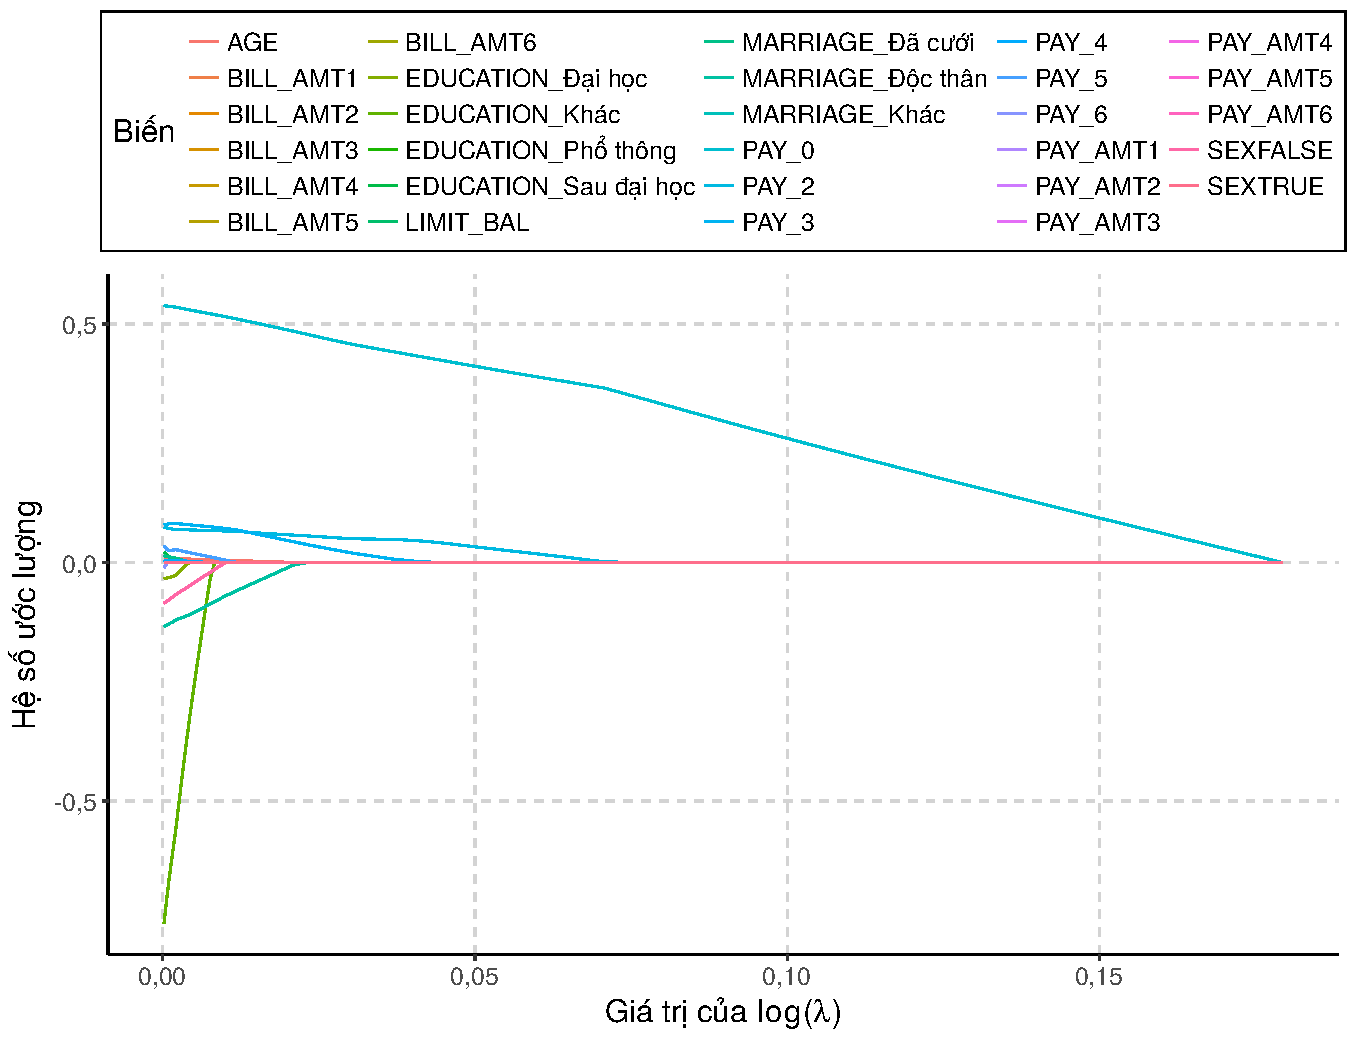
\includegraphics[width=\textwidth,height=12cm]{Figures/lasso_coef-1} 

\end{knitrout}
\caption{Giá trị ước lượng của các hệ số theo chiều tăng của $\log(\lambda)$}
\label{fig:lasso_coef}
\end{figure}

Hình \ref{fig:lasso_coef} mô tả xu hướng của các hệ số ước lượng $\beta$ khi giá trị của $\log\lambda$ thay đổi.
Với hướng tăng của $\log\lambda$ các biến thuộc nhóm \texttt{BILL} nhanh chóng hội tụ về $0$, thể hiện mức ý nghĩa thống kê thấp của các hệ số này trong mô hình. Trong khi đó, các biến thuộc nhóm \texttt{PAY} chậm hội tụ về $0$ hơn, với biến \texttt{PAY\_0} là biến cuối cùng có hệ số ước lượng $\beta$ tương ứng hội tụ về 0.
Với các giá trị $\lambda$ lớn hơn từ sau thời điểm này, có thể nói mô hình chỉ còn hệ số chặn $\beta_0$.

Để xác định giá trị hợp lý cho tham số $\lambda$ trong mô hình này. Chúng ta thực hiện bằng cách chia bộ số liệu thử nghiệm thành 10 phần nhỏ, chạy mô hình logit sử dụng phương pháp Lasso này trên từng bộ số liệu con này, rồi kiểm định kết quả mô hình dựa trên các bộ số liệu còn lại.
Từ kết quả của 10 phép ước lượng kiểm định chéo này, chúng ta có thể tính được giá trị trung bình của Deviance tại các giá trị của $\lambda$, qua đó chúng ta có thể xác định được giá trị của $\lambda$ mà Deviance là thấp nhất.

\begin{figure}
\centering
\capstart
\begin{knitrout}\small
\definecolor{shadecolor}{rgb}{0.969, 0.969, 0.969}\color{fgcolor}
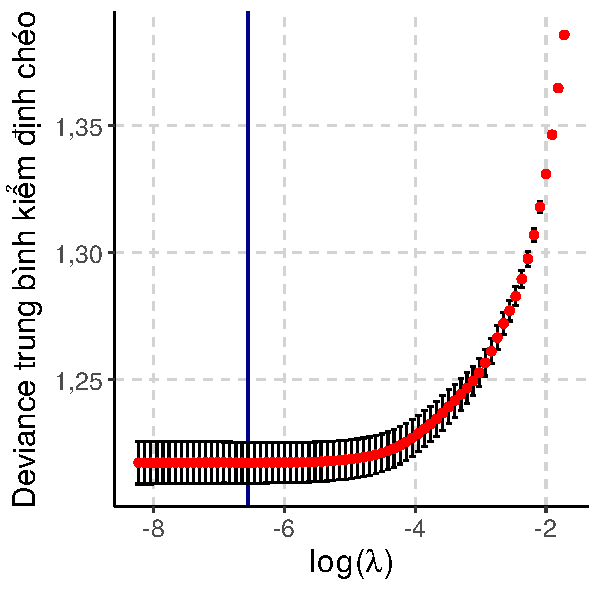
\includegraphics[width=10cm,height=10cm]{Figures/lasso_cv-1} 

\end{knitrout}
\caption{Giá trị trung bình của Deviance tương ứng với mỗi giá trị tương ứng của $\lambda$}
\label{fig:lasso_cv}
\end{figure}

Hình \ref{fig:lasso_cv} mô tả mối quan hệ của Deviance (trên trục tung) khi giá trị của $\lambda$ thay đổi (giá trị của $\lambda$ trên trục hoành đã được logarit hóa). Các chấm màu đỏ biểu diễn giá trị Deviance trung bình của kiểm định chéo tại các giá trị khác nhau của $\log(\lambda)$, thanh màu đen thể hiện sai số chuẩn tương ứng của giá trị trung bình này. Đường kẻ dọc màu xanh đậm đánh dấu giá trị của $\log(\lambda)$ mà tại đó gía trị của Deviance là thấp nhất($\lambda \approx\ $\text{0,001421}), tương đương với giá trị của $\lambda$ mà chúng ta lựa chọn cho mô hình này.

Hệ số ước lượng $\beta$ của mô hình được thể hiện trong bảng \ref{tab:lasso_final}). 

% latex table generated in R 3.3.3 by xtable 1.8-2 package
% Thu Apr 20 15:34:48 2017
\begin{table}[ht]
\centering
\begin{tabular}{rll}
  \hline
 & Tên biến & Hệ số \\ 
  \hline
1 & Hệ số chặn & 0,0488178 \\ 
  2 & LIMIT\_BAL & -7e-07 \\ 
  3 & SEXFALSE & -0,0741289 \\ 
  4 & EDUCATION\_Sau đại học & 0,0072849 \\ 
  5 & EDUCATION\_Đại học & -0,0296278 \\ 
  6 & EDUCATION\_Khác & -0,6249096 \\ 
  7 & MARRIAGE\_Đã cưới & 0,0109769 \\ 
  8 & MARRIAGE\_Độc thân & -0,1256848 \\ 
  9 & AGE & 0,008362 \\ 
  10 & PAY\_0 & 0,5365426 \\ 
  11 & PAY\_2 & 0,0705397 \\ 
  12 & PAY\_3 & 0,08174 \\ 
  13 & PAY\_4 & 0,0045188 \\ 
  14 & PAY\_5 & 0,0259231 \\ 
  15 & BILL\_AMT1 & -2e-06 \\ 
  16 & BILL\_AMT4 & 7e-07 \\ 
  17 & PAY\_AMT1 & -1,5e-05 \\ 
  18 & PAY\_AMT2 & -5,7e-06 \\ 
  19 & PAY\_AMT3 & -4,1e-06 \\ 
  20 & PAY\_AMT4 & -4,4e-06 \\ 
  21 & PAY\_AMT5 & -1,2e-06 \\ 
  22 & PAY\_AMT6 & -3,6e-06 \\ 
   \hline
\end{tabular}
\caption{Hệ số ước lượng} 
\label{tab:lasso_final}
\end{table}


\subsection{Kiểm tra hiệu quả của mô hình}


\begin{figure}
\centering
\capstart
\begin{knitrout}\small
\definecolor{shadecolor}{rgb}{0.969, 0.969, 0.969}\color{fgcolor}
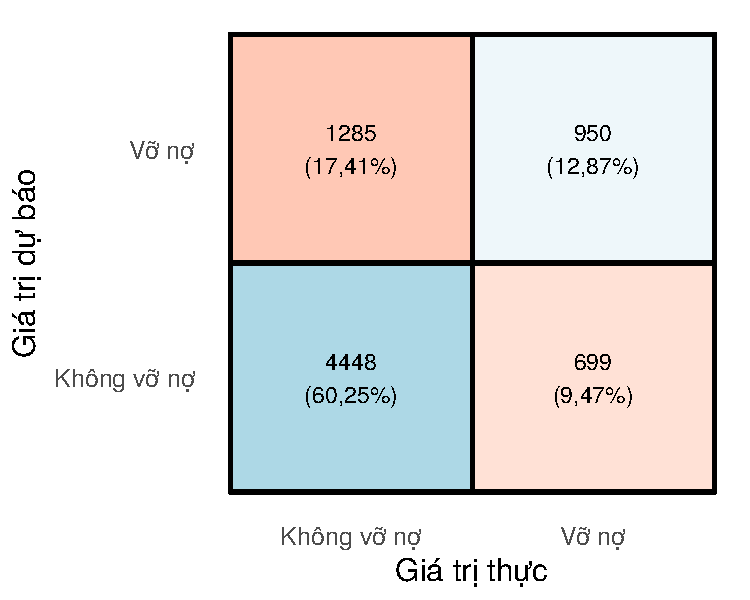
\includegraphics[width=10cm]{Figures/lasso_confusion_mat-1} 

\end{knitrout}
\caption{Confusion matrix cho mô hình logit (phương pháp Lasso)}
\label{fig:lasso_confusion_mat}
\end{figure}

Chúng ta sử dụng mô hình ước lượng được để dự báo trên tập số liệu kiểm tra. Hình \ref{fig:lasso_confusion_mat} minh họa một ma trận thể hiện độ chính xác của mô hình khi áp dụng lên tập số liệu kiểm tra, với màu xanh thể hiện các quan sát được dự đoán đúng và màu đỏ thể hiện các quan sát được dự đoán sai.

Trong tổng cộng \text{7382} dòng của bộ số liệu dùng để kiểm tra, có \text{1649} trường hợp vỡ nợ, trong đó mô hình dự đoán đúng \text{722} trường hợp. 
Đồng thời, trong các quan sát thuộc nhóm không vỡ nợ còn lại, có \text{519} quan sát bị mô hình đánh giá nhầm là có vỡ nợ.

Nhìn chung tỉ lệ dự đoán chính xác của mô hình trên tập số liệu kiểm tra là \text{80,41}\%, tỷ lệ của sai lầm loại I (không vỡ nợ nhưng mô hình dự đoán là có) là \text{7,03}\%, tỷ lệ của sai lầm loại II (có vỡ nợ nhưng dự đoán là không vỡ nợ) là \text{12,56}\%.


\section{Ứng dụng mô hình phân loại tuyến tính}

\section{Ứng dụng mô hình SVM}

%%%%%%%%%%%%
% Kết luận %
%%%%%%%%%%%%

\chapter{Kết luận}

%%%%%%%%%%%
% Phụ lục %
%%%%%%%%%%%
\appendix

\chapter{Thông tin về phiên làm việc trên R}

\begin{knitrout}\small
\definecolor{shadecolor}{rgb}{0.969, 0.969, 0.969}\color{fgcolor}\begin{kframe}


{\ttfamily\noindent\bfseries\color{errorcolor}{\#\# Error in system(paste(which, shQuote(names[i])), intern = TRUE, ignore.stderr = TRUE): cannot popen '/usr/bin/which 'uname' 2>/dev/null', probable reason 'Cannot allocate memory'}}\end{kframe}
\end{knitrout}

% \chapter{Code}



%%%%%%%%%%%%%%%%%%%%%%%
% Danh mục tham khảo  %
%%%%%%%%%%%%%%%%%%%%%%%
\printbibliography
\addcontentsline{toc}{chapter}{Tài liệu tham khảo}

\end{document}
